\documentclass[12pt]{article}
\usepackage[utf8]{inputenc}
\usepackage[T1]{fontenc}
\usepackage{hyperref}
\hypersetup{colorlinks=true, linkcolor=blue, filecolor=magenta, urlcolor=cyan,}
\urlstyle{same}
\usepackage{graphicx}
\usepackage[export]{adjustbox}
\graphicspath{ {./images/} }
\usepackage{amsmath}
\usepackage{amsfonts}
\usepackage{amssymb}
\usepackage[version=4]{mhchem}
\usepackage{stmaryrd}

\title{Report on Sublist3r}

\author{}
\date{}

\begin{document}
\maketitle
    Course No: CSE 406\\

    Course Title: Computer Security Sessional\\
    
    Presented By:

    Sadia Tabassum - 1905091

    Mayesha Rashid - 1905103

    Subsection: B2
\newpage

\section*{Table of Contents}
    \begin{enumerate}
        \item \hyperref[sec:subdomain-enumeration]{Subdomain Enumeration}
        \begin{enumerate}
            \item \hyperref[subsec:importance]{Importance}
            \item \hyperref[subsec:techniques]{Techniques}
            \item \hyperref[subsec:challenges]{Challenges}
            \item \hyperref[subsec:security-implications]{Security Implications}
            \item \hyperref[subsec:mitigation]{Mitigation}
        \end{enumerate}
        \item \hyperref[sec:sublist3r]{Sublist3r}
        \begin{enumerate}
            \item \hyperref[subsec:subbrute]{SubBrute}
        \end{enumerate}
        \item \hyperref[sec:high-level-overview]{High level Overview of Sublist3r}
        \begin{enumerate}
            \item \hyperref[subsec:brute-force]{Brute Force}
            \item \hyperref[subsec:search-engine]{Search Engine}
            \item \hyperref[subsec:dns-resolution]{DNS Resolution}
        \end{enumerate}
        \item \hyperref[sec:documentation]{Documentation to run each Feature}
        \begin{enumerate}
            \item \hyperref[subsec:installing-the-tool]{Installing the tool}
            \begin{enumerate}
                \item \hyperref[subsubsec:cloning-from-github]{Cloning from github}
                \item \hyperref[subsubsec:installation-on-linux]{Installation on Linux}
            \end{enumerate}
            \item \hyperref[subsec:running-the-tool]{Running the tool}
            \begin{enumerate}
                \item \hyperref[subsubsec:download-and-apply-patch-from-github]{Download and apply patch from github}
                \item \hyperref[subsubsec:setting-the-environment-variable]{Setting the environment variable}
            \end{enumerate}
            \item \hyperref[subsec:to-list-all-the-basic-options-and-switches-use-h-switch]{To list all the basic options and switches use -h switch:}
            \item \hyperref[subsec:to-enumerate-subdomains-of-specific-domain]{To enumerate subdomains of specific domain:}
            \item \hyperref[subsec:to-enumerate-subdomains-of-specific-domain-and-show-only-subdomains-which-have-open-ports-80-and-443]{To enumerate subdomains of specific domain and show only subdomains which have open\\
            ports 80 and 443:}
            \item \hyperref[subsec:to-enumerate-subdomains-of-specific-domain-and-show-the-results-in-realtime]{To enumerate subdomains of specific domain and show the results in realtime:}
            \item \hyperref[subsec:to-enumerate-subdomains-and-use-specific-engines-such-google-yahoo-and-virustotal-engines]{To enumerate subdomains and use specific engines such Google, Yahoo and Virustotal engines :}
            \item \hyperref[subsec:to-enumerate-subdomains-and-enable-the-bruteforce-module]{textTo enumerate subdomains and enable the bruteforce module:}
            \item \hyperref[subsec:usage]{Usage}
            \item \hyperref[subsec:using-sublist3r-as-a-module-in-python-scripts]{Using Sublist3r as a module in python scripts:}
            \item \hyperref[subsec:additional-tools-for-attempting-dictionary-attack]{Additional tools for attempting dictionary attack}
            \begin{enumerate}
                \item \hyperref[subsubsec:scout-installation]{Scout installation}
                \item \hyperref[subsubsec:chrome-driver-download]{Chrome driver download}
                \item \hyperref[subsubsec:chrome-driver-installation]{Chrome driver installation}
                \item \hyperref[subsubsec:burp-suite-installation]{Burp suite Installation}
            \end{enumerate}
        \end{enumerate}
        \item \hyperref[sec:exploring-sublist3r]{Exploring Sublist3r}   
        \begin{enumerate}
            \item \hyperref[subsec:subdomain-enumeration]{Subdomain Enumeration}
            \item \hyperref[subsec:specific-subdomains-enumeration]{Specific Subdomains Enumeration}
            \item \hyperref[subsec:attempting-a-dictionary-attack]{Attempting a dictionary attack}
            \begin{enumerate}
                \item \hyperref[subsubsec:subdomain-enumeration-of-vulnweb]{Subdomain Enumeration of vulnweb}
                \item \hyperref[subsubsec:finding-login-page-of-testphp.vulnweb.com]{Finding login page of \href{http://testphp.vulnweb.com}{testphp.vulnweb.com}}
                \item \hyperref[subsubsec:exploring-the-login-page-testphp.vulnweb.com-login]{Exploring the login page \href{http://testphp.vulnweb.com/login}{testphp.vulnweb.com//login}}
                \item \hyperref[subsubsec:running-the-attack]{Running the attack}
                \item \hyperref[subsubsec:attack-becomes-successful]{Attack becomes successful}
            \end{enumerate}
        \end{enumerate}
        \item \hyperref[sec:conclusion]{Conclusion}
    \end{enumerate}

\section{Subdomain Enumeration}\label{sec:subdomain-enumeration}
Subdomain enumeration is the process of identifying and cataloging the subdomains associated with a particular domain. Subdomains are subdivisions or additional components of a domain, typically represented as prefixes to the main domain name. It plays a crucial role in vulnerability analysis and web security.

\subsection{Importance}\label{subsec:importance}
\begin{itemize}
    \item \textbf{Discovery:} Identifying all possible subdomains associated with a domain.
    \item \textbf{Analysis:} Analyzing the structure and organization of subdomains to gain insights into the architecture of the target domain.
    \item \textbf{Security Assessment:} Subdomain enumeration helps security professionals identify potential points of entry, weaknesses, or misconfigurations in a domain's infrastructure.
    \item \textbf{Asset Management:} Maintaining an up-to-date inventory of all subdomains is essential for effective asset management. This ensures that organizations have a comprehensive understanding of their online presence and can take appropriate measures to secure it.
\end{itemize}

\subsection{Techniques}\label{subsec:techniques}
\begin{itemize}
    \item \textbf{DNS (Domain Name System) Interrogation:} Querying DNS records to identify subdomains associated with a domain.
    \item \textbf{Brute Force:} Systematically generating and testing possible subdomain names to discover valid ones.
    \item \textbf{Search Engine Scrutiny:} Leveraging search engines to identify publicly indexed subdomains.
    \item \textbf{Certificate Transparency Logs:} Analyzing certificate transparency logs to identify subdomains associated with SSL/TLS certificates.
\end{itemize}

\subsection{Challenges}\label{subsec:challenges}
\begin{itemize}
    \item \textbf{Incomplete Results:} DNS (Domain Name System) records may be cached, leading to incomplete or outdated information during subdomain enumeration. Some DNS servers may implement rate limiting, preventing exhaustive enumeration within a short time frame.
    \item \textbf{False Positives and Negatives:} Brute force techniques may yield false positives or negatives, leading to inaccurate results. The sheer volume of possible subdomains makes it challenging to ensure comprehensive coverage.
    \item \textbf{Dynamic Infrastructure:} Modern web applications and cloud-based services often have dynamic infrastructure, making it difficult to maintain an accurate and up-to-date inventory of subdomains.
\end{itemize}

\subsection{Security Implications}\label{subsec:security-implications}
Inability to accurately identify all subdomains may expose an organization to potential security threats, as attackers could target overlooked subdomains that lack robust security measures.

\subsection{Mitigation}\label{subsec:mitigation}
\begin{itemize}
    \item \textbf{Regular Enumeration:} Organizations should conduct regular subdomain enumeration to maintain an accurate inventory of their online assets.
    \item \textbf{Automation:} Leveraging automated tools and scripts to perform subdomain enumeration can help streamline the process and ensure comprehensive coverage.
    \item \textbf{Monitoring and Alerting:} Implementing mechanisms to detect changes in subdomain structure.
    \item \textbf{Security Measures:} Implementing robust security measures across all subdomains, including proper SSL/TLS configuration, secure coding practices, and regular vulnerability assessments, can help mitigate potential risks.
\end{itemize}

\section{Sublist3r}\label{sec:sublist3r}
Sublist3r is a subdomain enumeration tool written in python, designed to enumerate subdomains of a specific domain using OSINT. It is capable of leveraging multiple search engines, including Google, Yahoo, Bing, Baidu, and Ask, to identify subdomains associated with a target domain. Sublist3r also supports brute force enumeration using a wordlist, allowing users to discover additional subdomains that may not be indexed by search engines. It also uses Netcraft, Virustotal, DNSdumpster, and ReverseDNS to gather additional information about the target domain.

\subsection{SubBrute}\label{subsec:subbrute}
SubBrute is a free and open-source tool available on GitHub. It uses DNS Scan for finding subdomains of the target domain. It comes with Sublist3r by default. Sublist3r uses SubBrute for doing bruteforce search.

\section{High level Overview of Sublist3r}\label{sec:high-level-overview}
Sublist3r collects information of subdomains from various sources and then combines the results to provide a comprehensive list of subdomains. It uses the following techniques to gather information:

\subsection{Brute Force}\label{subsec:brute-force}
Sublist3r uses a wordlist to perform a brute force search for subdomains. It generates possible subdomain names and checks their existence by querying DNS records. This method is quite time consuming and may not always gather results due to rate limiting and other restrictions. The subbrute package is used for this method.

\subsection{Search Engine}\label{subsec:search-engine}
Sublist3r leverages multiple search engines, including Google, Yahoo, Bing, Baidu, and Ask, to identify subdomains associated with a target domain. It queries these search engines and scrapes the results to extract subdomains.

\subsection{DNS Resolution}\label{subsec:dns-resolution}
Sublist3r performs DNS resolution to verify the existence of subdomains. It queries DNS servers to resolve subdomain names and gather information about their IP addresses. It includes Netcraft, Virustotal, ThreatCrowd, DNSdumpster and ReverseDNS engines.

\section{Documentation to run each Feature}\label{sec:documentation}

\subsection{Installing the tool}\label{subsec:installing-the-tool}
\subsubsection{Cloning from github}\label{subsubsec:cloning-from-github}
git clone \href{https://github.com/aboul3la/Sublist3r.git}{https://github.com/aboul3la/Sublist3r.git}

\subsubsection{Installation on Linux}\label{subsubsec:installation-on-linux}
pip3 install -r requirements.txt

\subsection{Running the tool}\label{subsec:running-the-tool}
Virustotal engine of the tool doesn't work the way it used to during the creation of Sublist3r. To make it work, we need to update the base url of Virustotal. VirusTotal currently requires API key from their official website. We can get that by creating an account on their website. After getting the API key, we need to apply the patch from the github repository of Sublist3r.

\subsubsection{Download and apply patch from github}\label{subsubsec:download-and-apply-patch-from-github}
Patch link: \href{https://github.com/mehedi-imam241/sublist3r_patch_with_API_KEY/blob/main/changes.patch}{click here}

\subsubsection{Setting the environment variable}\label{subsubsec:setting-the-environment-variable}
The environment variable name has to be VT\_APIKEY. In Linux, open the .bashrc file in home directory and add the following line at the end of the file:

export VT\_APIKEY=your\_API\_key

Then save the file and run the following command in the terminal:\\
source ~/.bashrc

\subsection{To list all the basic options and switches use -h switch:}\label{subsec:to-list-all-the-basic-options-and-switches-use-h-switch}
python3 sublist3r.py -h

\subsection{To enumerate subdomains of specific domain:}\label{subsec:to-enumerate-subdomains-of-specific-domain}
python3 sublist3r.py -d example.com

\begin{center}
    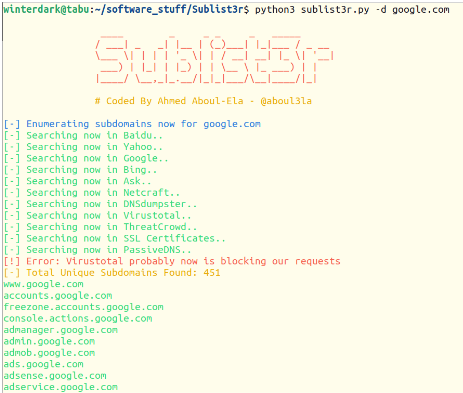
\includegraphics[max width=\textwidth]{Image1.png}
\end{center}

\subsection{To enumerate subdomains of specific domain and show only subdomains which have open ports 80 and 443:}\label{subsec:to-enumerate-subdomains-of-specific-domain-and-show-only-subdomains-which-have-open-ports-80-and-443}
python3 sublist3r.py -d example.com -p 80,443

\begin{center}
    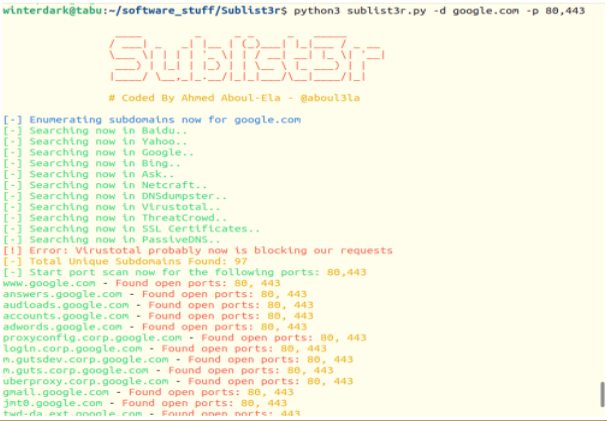
\includegraphics[max width=\textwidth]{Image2.png}
\end{center}

\subsection{To enumerate subdomains of specific domain and show the results in realtime:}\label{subsec:to-enumerate-subdomains-of-specific-domain-and-show-the-results-in-realtime}
python3 sublist3r.py -d example.com -v

\begin{center}
    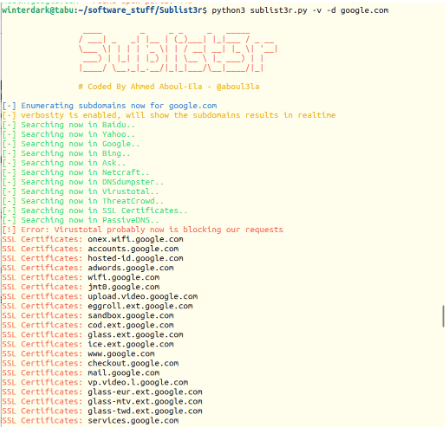
\includegraphics[max width=\textwidth]{Image3.png}
\end{center}

\subsection{To enumerate subdomains and use specific engines such Google, Yahoo and Virustotal engines :}\label{subsec:to-enumerate-subdomains-and-use-specific-engines-such-google-yahoo-and-virustotal-engines}
python3 sublist3r.py -d example.com -e google,yahoo,virustotal

\subsection{To enumerate subdomains and enable the bruteforce module:}\label{subsec:to-enumerate-subdomains-and-enable-the-bruteforce-module}
python3 sublist3r.py -d example.com -b

\subsection{Usage}\label{subsec:usage}
\begin{center}
    \begin{tabular}{c|c|c}
        \hline
        Short Form & Long Form & Description \\
        \hline
        -h & --help & show this help message and exit \\
        -d & --domain & Domain name to enumerate subdomains of \\
        -b & --bruteforce & Enable the subbrute bruteforce module \\
        -v & --verbose & Enable the verbose mode\\
        -p & --ports & Scan subdomains against specific tcp ports \\
        -e & --engines & Give a comma-separated list of search engines \\
        \hline
    \end{tabular}
\end{center}

\subsection{Using Sublist3r as a module in python scripts:}\label{subsec:using-sublist3r-as-a-module-in-python-scripts}
    import sublist3r \\
    subdomains = sublist3r.main(domain, no\_threads, savefile, ports, silent, verbose, enable\_bruteforce, engines) \\

    The main function will return a set of unique subdomains found by Sublist3r.

\subsection{Additional tools for attempting dictionary attack}\label{subsec:additional-tools-for-attempting-dictionary-attack}
Scout is a URL fuzzer for discovering undisclosed files and directories on a web server.

Hatch is a tool that is used to brute force most websites.

\subsubsection{Scout installation}\label{subsubsec:scout-installation}
curl -s "\href{https://raw.githubusercontent.com/liamg/scout/master/scripts/install.sh}{https://raw.githubusercontent.com/liamg/scout/master/scripts/install.sh}" | bash

\subsubsection{Chrome driver download}\label{subsubsec:chrome-driver-download}
Download chromedriver according to operating system from \href{https://googlechromelabs.github.io/chrome-for-testing/}{here}

\subsubsection{Chrome driver installation}\label{subsubsec:chrome-driver-installation}
Unzip the folder and add the directory to path variable. For Ubuntu, we have to add the following line to .bashrc file in home folder considering chromedriver folder is in home directory:

export PATH="\$PATH:/home/username/chromedriver/"

\subsubsection{Burp suite Installation}\label{subsubsec:burp-suite-installation}
Download link: \href{https://portswigger.net/burp/communitydownload} {https://portswigger.net/burp/communitydownload}

\section{Exploring Sublist3r}\label{sec:exploring-sublist3r}
\subsection{Subdomain Enumeration}\label{subsec:subdomain-enumeration}

To enumerate subdomains of \href{http://geeksforgeeks.com}{geeksforgeeks.com} using Google, Yahoo, and Virustotal engines, we can use the following command:\\
python3 sublist3r.py -d geeksforgeeks.com -e google,yahoo,virustotal

Running the command gives us the following output:

\begin{center}
    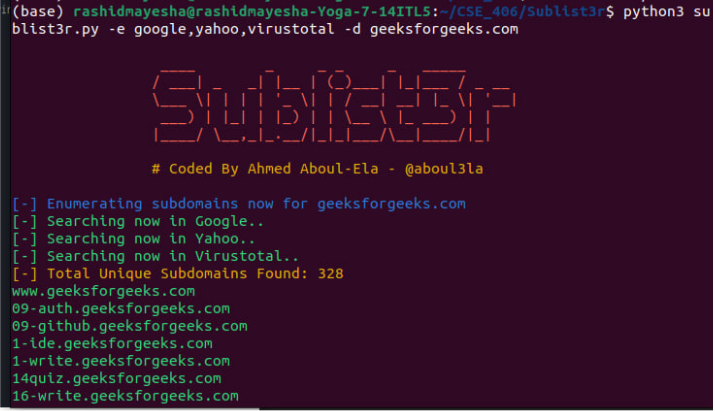
\includegraphics[max width=\textwidth]{Image4.png}
\end{center}

\subsection{Specific Subdomains Enumeration}\label{subsec:specific-subdomains-enumeration}
To show if some specific subdomains are available under a particular domain, we have to keep the list of desired subdomains in /subbrute/names.txt. For testing, we are keeping these six entries:

\begin{center}
    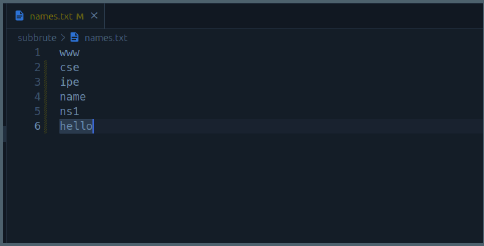
\includegraphics[max width=\textwidth]{Image5.png}
\end{center}

Then we can run the following command to check if these subdomains are available under \href{http://buet.ac.bd}{buet.ac.bd}:

python3 sublist3r.py -d buet.ac.bd -b

The output is as follows:

\begin{center}
    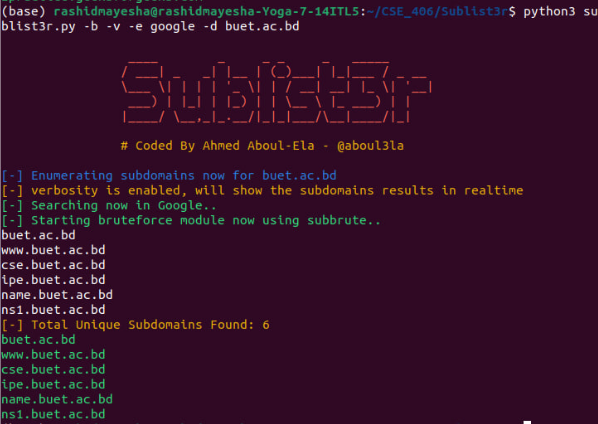
\includegraphics[max width=\textwidth]{Image6.png}
\end{center}

Subbrute lists domains and nameservers so we can see \href{http://buet.ac.bd}{buet.ac.bd}. Additionally, we can see that all other subdomains except hello is listed as it does not exist.

\subsection{Attempting a dictionary attack}\label{subsec:attempting-a-dictionary-attack}
\subsubsection{Subdomain Enumeration of vulnweb}\label{subsubsec:subdomain-enumeration-of-vulnweb}
Now we are going to attempt a dictionary attack on a vulnerable website. For safety reasons, we are running it on a safe website named vulnweb.

python3 sublist3r.py -e virustotal -d vulnweb.com

The output is as follows:

\begin{center}
    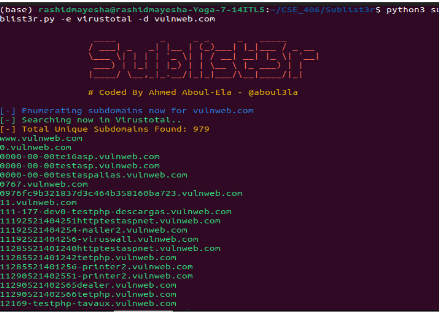
\includegraphics[max width=\textwidth]{Image7.png}
\end{center}

We see a subdomain with \href{http://testphp.vulnweb.com}{testphp.vulnweb.com}.

\begin{center}
    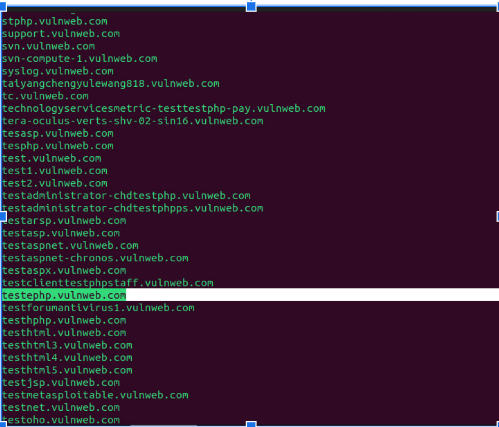
\includegraphics[max width=\textwidth]{Image8.png}
\end{center}

We are going to attempt a dictionary attack on this subdomain.

\subsubsection{Finding login page of \href{http://testphp.vulnweb.com}{testphp.vulnweb.com}}\label{subsubsec:finding-login-page-of-testphp.vulnweb.com}
We use scout to find out all the directories, subdirectories and files of \href{http://testphp.vulnweb.com}{testphp.vulnweb.com}. The command is as follows:\\
scout url http://testphp.vulnweb.com

The output will look like:

\begin{center}
    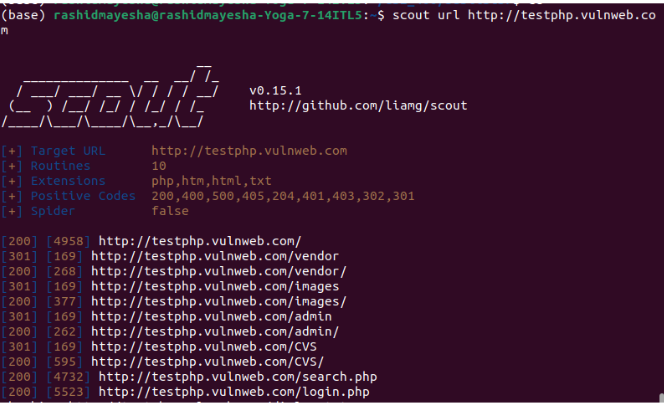
\includegraphics[max width=\textwidth]{Image9.png}
\end{center}

We see that there is a login page at \href{http://testphp.vulnweb.com/login}{testphp.vulnweb.com/login}. We are going to attempt a dictionary attack on this page.

\subsubsection{Exploring the login page \href{http://testphp.vulnweb.com/login}{testphp.vulnweb.com//login}}\label{subsubsec:exploring-the-login-page-testphp.vulnweb.com-login}

\begin{center}
    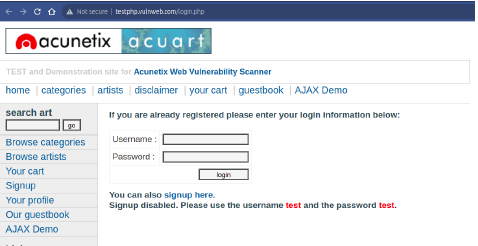
\includegraphics[max width=\textwidth]{Image10.png}
\end{center}

If we paste the link in browser, we can see that the page is alive.

\subsubsection{Running the attack}\label{subsubsec:running-the-attack}
Now let's create a new project in burp suite and turn the intercept on in proxy field. From there, we will click the open browser, which will open burp suite's browser. There we will open the login page and try to login with some random credentials. We will see the request in burp suite.

\begin{center}
    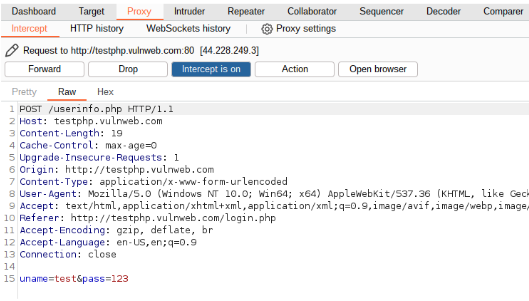
\includegraphics[max width=\textwidth]{Image11.png}
\end{center}

Now we will send this request to intruder and add password as payload by adding curly braces (§) on either side.

\begin{center}
    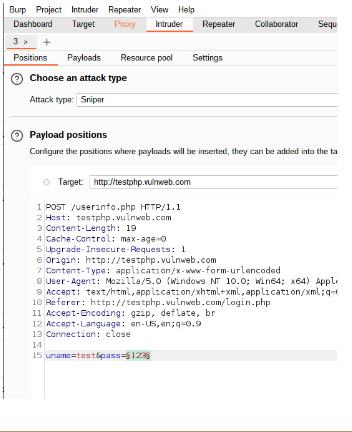
\includegraphics[max width=\textwidth]{Image12.png}
\end{center}

In payloads, we load our password lists file and click start attack.

\begin{center}
    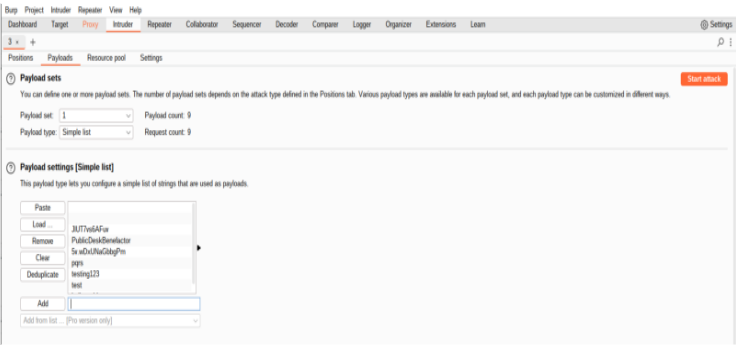
\includegraphics[max width=\textwidth]{Image13.png}
\end{center}

\subsubsection{Attack becomes successful}\label{subsubsec:attack-becomes-successful}
From the attack we can see that, for password test we have got status code 200 and the length is different than others. We now select the request of test and forward it to repeater.

\begin{center}
    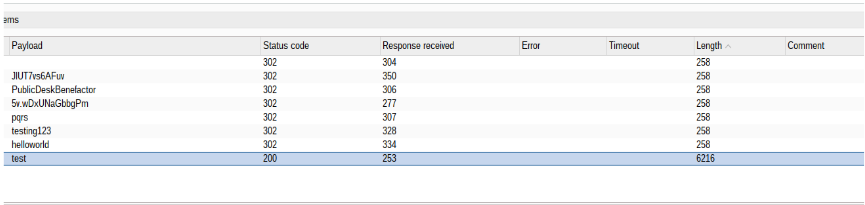
\includegraphics[max width=\textwidth]{Image14.png}
\end{center}

If we click send at repeater, we will see that we get a webpage as a response. Now copying this request to proxy and forwarding it will load the logged in page in browser. Thus a successful dictionary attack has been done.

\begin{center}
    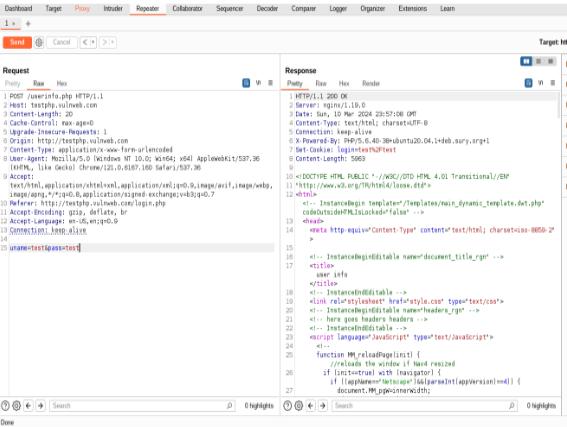
\includegraphics[max width=\textwidth]{Image15.png}
\end{center}

\begin{center}
    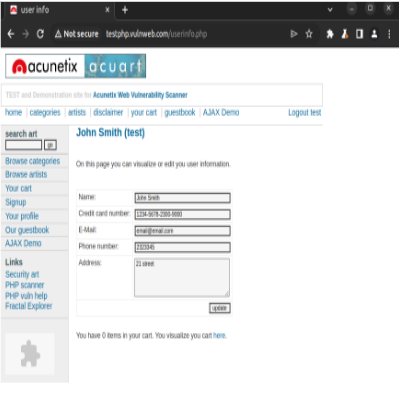
\includegraphics[max width=\textwidth]{Image16.png}
\end{center}

\section{Conclusion}\label{sec:conclusion}
Therefore, we can say that Sublist3r is a powerful tool for subdomain enumeration. It can be used to find subdomains of a specific domain using various search engines and DNS resolution. It also supports brute force enumeration using a wordlist. Sublist3r can be used to identify potential points of entry, weaknesses, or misconfigurations in a domain's infrastructure. It is an essential tool for vulnerability analysis and web security.

\end{document}